\documentclass[range]{ar2e}
       
\usepackage{amsmath}
\usepackage{color}
\usepackage{verbatim}
\usepackage{graphicx}
\usepackage{wasysym}
\usepackage{amssymb}

\begin{document}

\input epsf.def
\input psfig.sty

%\jname{Annual Review of Condensed Matter Physics}
%\jyear{2012}
%\jvol{XX}
%\ARinfo{1056-8700/97/0610-00}

\title{Designer Hamiltonians---bridging lattice-scale physics and continuum field theory with 
quantum Monte Carlo simulations} 

\author{Ribhu K. Kaul
\affiliation{Department of Physics and Astronomy, University of Kentucky, Lexington, Kentucky 40506, USA}
Roger G. Melko
\affiliation{Department of Physics and Astronomy, University of Waterloo, Ontario, N2L 3G1, Canada, and
Perimeter Institute for Theoretical Physics, Waterloo, Ontario N2L 2Y5, Canada}
Anders W. Sandvik
\affiliation{Department of Physics, Boston University, 590 Commonwealth Avenue, Boston, Massachusetts 02215, USA}}

\begin{abstract}
We discuss designer Hamiltonians---lattice models tailored to be free from sign problems (``de-signed'') when simulated with quantum 
Monte Carlo methods but still host complex  many-body states and quantum phase transitions of great interest in condensed matter 
physics. We focus on quantum spin systems in which competing interactions lead to non-magnetic ground states. These states and 
associated quantum phase transitions can be studied in great detail, enabling direct access to universal properties and connections 
to be made with low-energy effective quantum field theories. As specific examples, we discuss the transition from a N\'eel antiferromagnet to 
either a uniform quantum paramagnet or a spontaneously symmetry-broken valence-bond solid in SU($2$) and SU($N$) spin models. We also 
discuss anisotropic (XXZ) systems harboring topological Z$_2$ spin liquids and the XY$^*$ transition. We briefly review recent progress 
on quantum Monte Carlo algorithms, including ground state projection in the valence-bond basis and direct computation of the Renyi variants of the 
entanglement entropy.
\end{abstract}

\maketitle

\section{Introduction}
\label{sec:intro}

Quantum field theory is a powerful framework for studies of low-energy properties of complex strongly 
correlated and entangled quantum matter systems \cite{Sachdev11}. There are potential pitfalls and difficulties 
with this approach, however, and it is, therefore, important to also investigate systems directly based on the Hamiltonian 
formulation. One of the most fruitful directions is to use numerical methods to study lattice Hamiltonians 
in an unbiased way, and to extract from such calculations emergent low-energy properties which can be 
compared with results for corresponding quantum field theories. Such connections between the two approaches 
can have significant synergy effects in advancing our understanding of quantum many-body phenomena---as they
have had and continue to have in classical statistical mechanics, especially in studies of phase transitions. 

Computational research has its own challenges, however, and many quantum models of interest are currently beyond the reach 
of existing algorithms. Frustrated quantum spin systems and fermions in two and three dimensions are the two main groups 
of difficult systems. They are generally associated with the infamous ``sign problem'' in quantum Monte Carlo (QMC) simulation
\cite{Loh90,Henelius00,Nyfeler08}, i.e., the weight function in the configuration space constructed using the Euclidean path 
integral or other mappings to an effective statistical-mechanics problem is not positive definite (and hence cannot be directly 
used as a probability distribution for importance sampling). The approach we advocate and review here is to construct particular 
``designer hamiltonians'', which host interesting ground states and quantum phase transitions but still are amenable to 
large-scale QMC studies without sign problems (i.e., they are ``de-signed'' by design). 

A common misconception is that interesting designer Hamiltonians should not exist---if a model is sign-problem 
free it must be trivial or uninteresting. There are already many counter-examples to this pessimistic view, 
however, and we will here review some recent examples from the area of quantum magnetism. Advances in QMC 
methods \cite{Sandvik91,Evertz93,Beard96,WormA,Sandvik99,Sandvik10a} have made it possible to truly approach the 
low-energy limit of many important models without any approximations (beyond controllable statistical errors), and to compute 
quantities of great current interest in condensed matter physics and quantum information theory, e.g., the fidelity 
\cite{Schwandt09,Degrandi11} and the entanglement entropy \cite{Hastings10, Melko10}. We will brifly address some of these technical 
aspects as well. We here first give some further remark on field theory and the philosophy of the synergistic use of 
designer Hamiltonians, and then outline the topics covered in this review.

\subsection{Field theory and numerical studies of Hamiltonians}

A field theory can rarely be rigorously derived exactly from 
an underlying Hamiltonian (which is the natural starting point for describing condensed matter systems). Instead
it is constructed based on symmetries, in combination with insights or assumptions on the physical nature of the
system. Some times the field theory can be derived in some well defined limit, e.g., the $(d+1)$-dimensional
nonlinear $\sigma$-model description of interacting quantum spins in $d$ dimensions was derived by Haldane in 
the semi-classical limit of large spin $S$ by using coherent spin states \cite{Haldane83,Chakravarty89,Auerbach94}. 
In other cases, the field theory is constructed heuristically, e.g., the non-compact CP$^{N-1}$ action
proposed to describe the intriguing ``deconfined'' quantum-critical point in $d=2$ quantum magnets with 
transitions between a N\'eel antiferromagnet and a valence-bond solid (VBS) \cite{Senthil04a,Sachdev08}.

%It is
%not {\it a priori} clear whether the mapping is correct for all $d$ and small $S$, although it is now well
%established that it is for the Heisenberg chain ($d=1$) for any $S$. The $d=2$ Heisenberg model and certain
%transitions out of its N\'eel antiferromagnetic ground state is also believed to be captured by this field
%theory for any $S$ \cite{Chakravarty89}. 

Having identified or proposed a field
theory, the next step is to extract its properties. This is typically done using the renormalization group (RG)
approach, which may result in flows to some previously known fixed point, or to some fixed point or effective
model whose properties are not known. The RG itsef may have to rely on approximations that are not always easy
to justify, and if the flow is to some unknown state, it may be challenging to characterize it. Often the theory
is modified in such a way that it can be rigoroulsy controlled and the physical situation of interest is studied 
by some expansion around it. Well known examples are the $\epsilon$ expansion around the upper critical dimension 
and the $1/N$ expansion in the number of components $N$ (spin components, flavors of fermions, etc). The
extrapolation to the $\epsilon$ or $N$ of main interest is often challenging, however, because only low-order
expansions are feasible in practice.

Because of issues such as these, it is important to test the predictions of field theories in some unbiased way
starting from a microscopic description of the system or phenomenon of interest. In some cases there are exact solutions, 
e.g., the Bethe Ansatz solution of the $S=1/2$ Heisenberg chain \cite{Bethe31} has been immensely important for testing 
the non-linear sigma model description of this class of critical spin chains. The exact AKLT state \cite{affleck88} for a special 
version of the $S=1$ chain was similarly important in testing Haldane's prediction of the qualitative differences between 
half-odd integer and integer spins \cite{Haldane83}. Exact solutions are rare, however, and essentially limited to 1D models. 
Another, more general approach is to study Hamiltonians numerically. Exact diagonalization of the Hamiltonian is possible 
only for very small systems; currently up to $\approx 42$ $S=1/2$ spins \cite{Nakano11,Lauchli11}. White's density matrix 
renormalization (DMRG) scheme \cite{White92} and related approaches based on matrix-product states \cite{Schollwock05} 
have enabled even more detailed studies of the low-energy physics of 1D systems (including also ``ladders'' of several 
coupled chains). While there has been some progress for 2D systems, with DMRG \cite{Stoudenmire12} and tensor-product 
\cite{Murg09} states (generalizations of matrix-product states), in general these approaches have not yet reached the 
level where one can obtain unbiased results for large systems.

The only numerical approach with which one can reach sufficiently large lattices in two and three dimensions is QMC 
simulations \cite{Evertz03,Sandvik10b}, and, as already noted, they are often limited in practice by sign problems. The 
class of models for which there is no sign problem, or it is known how to circumvent it, still contains a vast range of 
models with non-trivial and interesting ground states and quantum phase transitions. To study low-energy emergent 
properties, the interactions do not necessarily have to correspond closely to any particular material (although some 
times that is also possible). The idea is to design a sign-problem free Hamiltonian in such a way that it contains a 
particular macroscopic (low-energy) phenomenon of interest---so that universal physics is captured. With unbiased large-scale 
QMC simulations of such designer hamiltonians one can test field theories proposed to capture specific quantum many-body 
states or quantum phase transitions. Moreover, explorations of designer hamiltonians can also serve as ``experiments'' 
for discovering novel phenomena, and, thereby, stimulate further theoretical developments.

Note that the notion of designer Hamiltonians we consider here goes beyond the often used approach of investigating quantum phenomena 
in $d$ dimensions by simply extending the same model to $d+1$ dimensions. While this works in some cases \cite{Rieger94,Sorensen92,Nahum11}, 
it has in recent years been realized that this approach can miss important and intriguing quantum states that have no natural or familiar 
classical analogues based just on a simple order parameter \cite{Senthil04a,Fradkin04,Sachdev08}. While a designer Hamiltonian effectively also {\it is} 
a classical statistical-mechanics model (which arises out of the construction of the sampling space in the QMC scheme implemented), it is 
often not one that would have come natural as a starting point just from the perspective of increasing the dimensionality of some
classical model. Note, in particular, that it is now well established that symmetries alone do not uniquely determine the nature of a 
quantum phase transition, but systems with the same symmetries can belong to different universality classes, depending on the role of topological 
defects \cite{Motrunich04}. Thus, in our view the approach of using manifestly quantum mechanical designer Hamiltonians is an important direction
in research on many-body ground states, quantum criticality, and other emergent phenomena.

\subsection{Outline of the Review}

In this review, we will focus on some recent concrete examples where it has been possible to study quantum phase transitions in detail 
by QMC studies, and to make contact with corresponding field theories by, e.g., comparing analytical and numerical results for critical 
exponents. We also discuss other fascinating quantum phenomena, e.g., emergent gauge fields and entanglement, where QMC studies are
playing a critical role in establishing bench-marks and gaining insights that are hard or impossible to exctract from the field theories.

In Sec.~\ref{sec:methods} we discuss the sign problem and some of the QMC schemes used in large-scale studies of quantum spin systems, 
including treatments of SU($N$) symmetry and recent progress in computing the Renyi entanglement entropy. In Sec.~\ref{sec:su2models} 
we give examples of conventional and deconfined quantum-critical points in SU(2) invariant models, and in Sec.~\ref{sec:sunmodels} 
we show how generalization to SU($N$) symmetry can be used to directly connect to large-$N$ studies within field theory. In Sec.~\ref{sec:u1models} 
we discuss spin liquid states and associated quantum phase transitions in U($1$) symmetric ``XXZ'' spin models (or, equivalently, hard-core bosons). 
We conclude in Sec.~\ref{sec:discussion} with a discussion of future prospects and challenges.

\section{Modern QMC methods}
\label{sec:methods}

There is a wide range of QMC methods available for studies of different classes of models \cite{Assaad07,Evertz03,Sandvik10b}. In this review we 
focus on spin models, and therefore restrict the discussion to the types of methods most suitable for them. These methods are also often well suited 
for studies of bosons, where a substantial body of work has been carried out in the last few years stimulated by ultracold atoms in optical lattices. 
For fermions, other approaches work much better in practice (except for 1D systems, where the methods discussed here also work well since the 
signs from anticommutation normally do not appear in this geometry). We will here only give a rough overview of the methods.

\subsection{The sign problem}
\label{ss:sign}

Solving many-body quantum mechanical problems on a computer is {\em generally} exponentially hard (in computing time versus system size) 
with known algorithms. The statistical mechanics of a $d$-dimensional quantum Hamiltonian can be rewritten in terms of some classical variables 
$C$ in $d+1$ dimensions, e.g., the partition function ($T>0$) or the normalization ($T=0$) has the form
\begin{equation}
\label{eq:wc}
Z=\sum_C W_C.
\end{equation}
Systems of interest can, for practical, known ways of transforming into the above form, have positive and negative weights $W_C$, 
invalidating the usual interpretation of $W_C/Z$ as a probability distribution in Monte Carlo simulations. Formally, this difficulty 
can be side-stepped by not including the sign in the probability $P_C \propto |W_C|$ and compensating by weighting the observables with it;
\begin{equation}
\langle O \rangle = \frac{\sum_C W_C O_C}{\sum_C W_C} =
\frac{\sum_C O_C {\rm Sign}(W_C) |W_C|}{\sum_C {\rm Sign}(W_C)|W_C|} = 
\frac{\langle {\rm Sign} \cdot O\rangle_{|W|}}{\langle {\rm Sign}\rangle_{|W|}}.
\label{expvalue}
\end{equation}
The problem here is that the numerator and denominator in the last expression both approach zero
exponentially in system size and inverse temperature, and, hence, resolving (\ref{expvalue})
within statistical noise is exponentially hard. The advantage of importance sampling (time speed-up 
from exponential to polynomial scaling) is then lost. This predicament is the QMC sign problem.

We here consider classes of quantum Hamiltonians for which it is possible to choose a basis in which all 
the $W_C\geq 0$. These sign-problem free models can generally be simulated in polynomial time by 
importance sampling, allowing access to large system sizes (with the exception of ``glassy'' systems and
other systems where even classical Monte Carlo simulations scale exponentially). In some cases, sign problems
can be solved in more sophisticated ways, e.g., in the Meron algorithm \cite{Chandrasekharan99}. Here we 
implicitly consider cases where the ``de-signing'' is essentially automatic, being related to the bipartiteness 
of the interactions.
 
\subsection{$T>0$ and $T=0$ QMC methods}
\label{ss:method}

In {\it finite-temperature} methods, the goal is to compute thermal averages
\begin{equation}
\langle A\rangle = \frac{1}{Z}{\bf Tr}\{ {\rm e}^{-\beta H}\},~~~
Z = {\bf Tr}\{ {\rm e}^{-\beta H}\},
\label{za1}
\end{equation}
where $\beta=1/T$. As an alternative to studying the ground state in the limit of  $T\to 0$, in a {\it ground-state projector} method some 
operator $P(\beta)$  is applied to a ``trial state'' $|\Psi_0\rangle$, such that $|\Psi_\beta \rangle = P(\beta)|\Psi_0\rangle$ approaches the 
ground state when $\beta \to \infty$. An expectation value
\begin{equation}
\langle A\rangle = \frac{1}{Z}\langle \Psi_\beta|A|\Psi_\beta\rangle,~~~~ Z = \langle \Psi(\beta)|\Psi(\beta)\rangle,
\label{za2}
\end{equation}
tends to the true ground state expectation value, $\langle A\rangle$ $\to$ $\langle 0| A|0\rangle$. For the projector, one can use the imaginary-ime
evolution operator $P(\beta)={\rm e}^{-\beta H}$ or a high power of the hamiltonian, $P(m)=H^m$. Here $m \propto \beta N$ gives the same rate of 
convergence for the two choises for a given system size $N$. This follows from a Taylor expansion of the time evolution operator, which for large 
$\beta$ is dominated by powers of the order $n=\beta |E_0|$, where $E_0$ is the ground state energy (which is proportional to $N$).

\subsection{Path integrals and stochastic series expansion}

The task is now to rewrite $Z$ in (\ref{za1}) or (\ref{za2}) into the form (\ref{eq:wc}), and expectation values as (\ref{expvalue}), with classical variables 
without diagonalizing $H$. In practice, implementations of $T=0$ and $T>0$ approaches for a given model are often very similar. In either case, the exponential 
operator can be treated with path-integral methods---world lines in discrete \cite{Suzuki77,Hirsch82} or continuous \cite{Beard96,Prokofev96,Prokofev98} 
imaginary time---starting from a product of ``time slices'',
\begin{equation}
{\rm e}^{-\beta H}= \prod_{i=1}^M {\rm e}^{-\Delta H},~~~~ \Delta=\frac{\beta}{M}.
\label{slicing}
\end{equation}
Complete sets of states are inserted between the exponentials (and the trace is further taken at $T>0$). For small $\Delta$, the
matrix elements of the exponentials can be evaluated approximately, giving the form (\ref{eq:wc}) with $W_C$ a product of $M$ matrix elements. 
In modern approaches the limit $\Delta \to 0$ is taken at the algorithmic level \cite{Prokofev96,WormA,Beard96} and the Monte Carlo sampling is of 
paths in continuous imaginary time. Older approaches employed the Suzuki-Trotter decomposition \cite{Suzuki76} in Eq.~(\ref{slicing}), which 
typically leads to an error $\mathcal{O}(\Delta^2)$.

An alternative way is to start from a series expansion \cite{Handscomb62,Sandvik91},
\begin{equation}
{\rm e}^{-\beta H}= \sum_{n=0}^\infty \frac{\beta^n}{n}(-H)^n,
\label{series}
\end{equation}
and inserting complete sets of states between each instance of $H$. The power $n$ itself is importance-sampled along with the terms of $H$ 
(stochastic series expansion; SSE), and the expansion is sharply peaked around $\langle n\rangle = -\beta E_0$ (under the assumption that there 
is no sign problem). Again, $W_c$ in (\ref{eq:wc}) is a product of matrix elements. The continuous-time path integral can also be seen as a variant 
of SSE, where the evolution operator is written in the interaction picture, with $H=H_0+V$ and expanding only in $V$ \cite{Prokofev96,Sandvik97a}. 
The full SSE is normally more efficient for spin systems, while the continuous-time variant should be better for certain boson systems.

Regardless of how the exponential operator is treated, the difference between Eqs.~(\ref{za1}) and (\ref{za2}) is essentially only in the boundary 
conditions in the imaginary time direction; periodic for $T>0$ (due to the trace being taken) and dictated by the nature of the trial state in $T=0$ 
projections. An equal superposition over all basis states corresponds to fully open boundaries, while other choices of the trial state leads to open 
boundaries (with some weighting of the bra and ket states, depending on the details of the trial state). 

There is no sign problem in these approaches for spin systems on bipartite lattices (for a properly chosen trial state in the case of the $T=0$ approach); 
essentially because there is always an even number of the negative matrix elements in $W_C$, or, equivalently, all of them can be rendered positive by a 
sublattice transformation. For details, see, e.g., Ref.~\cite{Henelius00}.

\subsection{Sampling with loop and cluster algorithms}

A break-throug leading to today's efficient QMC algorithms of the types discussed above
was the realization \cite{Evertz93} that generalizations of the classical Swendesn-Wang (SW) cluster 
Monte Carlo method \cite{Swendsen88} could be generalized to loop algorithms (i.e., clusters in the form of one-dimensional loops) for vertex models, and that 
these vertex models are very similar to the effective statistical mechanics problems arising in the transformations of the quantum problem discussed above. Such 
loop algorithms cannot be applied to all cases (in analogy with the SW method, which also has limited applicability), but the loop concept has also been further 
generalized to ``worms'' \cite{Prokofev96,Prokofev98, WormA} and ``directed loops'' \cite{Sandvik99,Syljuasen02}, which are essentially loops that can self-intersect
during their construction and incorporate the detailed-balance principle in a more general way. Recently such an algorithm was also formulated without
delatiled balance \cite{Suwa10}. In addition, for some models where loop algorithms and their generalizations are not applicable (e.g., transeverse-field 
Ising models), other efficient generalizations of the SW concept have been developed \cite{Rieger99,Sandvik03}.

\subsection{Special techniques for SU(2)-symmetric models}

A particularly convenient class of trial states in projector QMC with SU($2$) invariant interactions is the amplitude-product states in the valence-bond
(singlet pair) basis \cite{Liang88}, which were recently generalized to include bond correlations \cite{Lin12}. These overcomplete states for the singlet 
sector incorporate Marshall's sign rule in a convenient way and also automatically have the appropriate momentum for the ground state of a periodic system 
(thereby from the outset filtering out a significant fraction of the excited states). The hamiltonian in this case can typically be expressed in terms of 
two-spin singlet-projector operators  (individual ones or products of two or more of them);
\begin{equation}
P_{ij}=\hbox{$\frac{1}{4}$}-{\bf S}_i\cdot {\bf S}_j = |s_{ij}\rangle\langle s_{ij}|,
\label{psinglet}
\end{equation}
where $s_{ij}$ denotes the singlet state of spins $i$ and $j$. A power of the Hamiltonian $H^m$, for fixed $m$ or in a series expansion, Eq.~(\ref{series}),
is expanded into all possible products of these projectors, which act on the ket trial state in (\ref{za2}). In early versions of this scheme, the resulting 
paths of valence bond states were sampled \cite{Liang90,Santoro99,Sandvik05}, while in more recent formulations the diagonal and off-diagonal parts of the 
projectors are also sampled, along with spin configurations compatible with the valence-bond configurations of the trial state (which are also sampled) 
\cite{Sandvik10c}. An example of a configuration in such a simulation is shown in Fig.~\ref{loops}. This configuration space is amenable the very efficient 
loop updates discussed above \cite{Sandvik10a}. Apart from the boundary conditions in the ``propagation'' direction (and the associated sampling of the
valence bonds in the trial state), this kind of projector method is in practice implemented in a very similar way as the SSE method for SU($2$) 
models \cite{Sandvik10b}.

\begin{figure}
\centerline{\psfig{figure=loops.eps,height=4.5cm}}
\caption{A configuration in a valence-bond projector simulation of a 4-site Heisenberg chain; here with a small projection power, 
$m=2$ \cite{Sandvik10a}. The vertical bars indicate singlet-projectors operators, while the arcs on the left (bra) and right (ket) represent 
valence bond configurations of the sampled trial state. Open and closed circles indicate up and down spins, which are unchanged between 
operators and represented by horizontal lines there. These lines, along with the valence bonds, form loops that can be flipped (i.e., 
all spins traversed by the loop are flipped) without changing the configuration weight. A configuration in a $T>0$ simulation corresponds 
to imposing periodic boundary conditions in the ``time'' direction, instead the independent boundaries terminated by valence bonds.}
\label{loops}
\end{figure}

Evaluation of expectation values (``measurements'') in projector QMC simulations are carried out at the mid-point of the configuration, as indicated 
in Fig.~\ref{loops}. In the valence-bond basis, when propagating the bra and ket states in the pure valence-bond basis (which corresponds to averaging 
over all compatible spin configurations), most quantities of interest can be expressed using the loops of the transition graph formed when superimposing 
the projected bra and ket states. Estimators for various correlation functions are discussed in Refs.~\cite{Beach06} and \cite{Tang11a}.

\subsection {Generalizations from SU(2) to SU(N)}
\label{ss:su2N}

The above methods for SU(2) can be extended to a certain
class of spin models with an SU($N$) symmetry on bipartite
lattices. We can proceed by first recognizing that the Heisenberg operator is simply a singlet projector, $P_{ij}=\hbox{$\frac{1}{4}$}-{\bf S}_i\cdot {\bf S}_j = |s_{ij}\rangle\langle s_{ij}|$.
In order to generalize this operation to SU($N$), we choose models that have an SU($N$) spin with a
fundamental representation on the A sub-lattice and an SU($N$) spin with
a conjugate to fundamental representation on the B sub-lattice~\cite{affleck1985:lgN,Read89}.
Denoting the $N$ states on each site of our lattice by $|\alpha\rangle$ where
$1\leq \alpha \leq N$ 
and the generators of the fundamental representation by $T^a$ (an
$N\times N$ matrix),
the SU($N$) singlet between a spin $i$ on the A sub-lattice and a spin $j$ on the
B sub-lattice is given by, $|s^N_{ij}\rangle = \frac{1}{\sqrt{N}}\sum_\alpha
|\alpha_i\alpha_j\rangle$. We can use this state to rewrite the
manifestly SU($N$) invariant interaction  $\sum_a T^a_i \cdot
T^{*a}_j$, as an explicitly sign problem free projection operator,
\begin{equation}
\sum_a T^a_i \cdot
T^{*a}_j + \frac{1}{N^2} = |s^N_{ij}\rangle \langle s^N_{ij}|\equiv P_{ij}
\end{equation}
This is an SU($N$) invariant generalization of the SU(2) Heisenberg interaction
for two spins on {\em opposite} sub-lattices. Another interaction of interest is an SU($N$) invariant interaction
between sites having the same representation, the permutation
operator, which is defined by its action on a ket,
$\frac{\Pi_{ij}}{N}|\alpha_i\beta_j\rangle \equiv |\beta_i\alpha_j\rangle$. We can now relate this operator to the generators $T^a$,
\begin{equation}
\sum_a T^a_i \cdot
T^{a}_j +\frac{1}{N^2} =\Pi_{ij}
\end{equation}
This is an SU($N$) invariant generalization of the SU(2) Heisenberg
interaction for two spins on the {\em same} sub-lattice.
In terms of the definitions of $P_{ij}$ and $\Pi_{ij}$, the algorithms presented in
Sec.~\ref{ss:method} can be generalized from SU(2) to SU($N$) by
extending the number of loop colors from 2 to $N$~\cite{harada2003:sun,beach2009:sun,kaul2011:j1j2}.


\subsection{Renyi entropies in $T=0$ and $T>0$ simulations} 
\label{ss:renyi}


In addition to conventional estimators discussed in Equations \ref{za1} and \ref{za2}, QMC methods have recently been developed that are capable of measuring estimators related to the {\it entanglement} of a quantum system \cite{EntangleMeasure}.  Several quantities related to entanglement have been explored in a QMC context for their abilities to identify and characterize quantum phases and phase transitions
\cite{Tommaso1,Tommaso2,fluc1,fluc2,fid1,fid2}.  In this review, we concentrate of measures of the entanglement entropy, specifically the {\it Renyi} entropies \cite{renyi},
\begin{equation}
S_{\alpha} = \frac{1}{1-\alpha} \ln \Big[ {\rm Tr}\big( \rho_A^{\alpha} \big) \Big]
\end{equation}
which are defined for integer $\alpha \ge 1$.  Here, $\rho_A$ is the reduced density matrix, $\rho_A = {\rm Tr}_B (\rho)$, and $A$ is a subregion of a lattice system (with $B$ being its complement).  
 
The direct measure of Renyi entropies is not possible in QMC using conventional estimators, however recent work has demonstrated that it is possible to measure $S_{\alpha}$ using a {\it replica trick} \cite{Holz,Cardy, Fradkin, BP, Naka}.  Here, $\alpha$ copies of the simulation cell are used, with modified periodic boundaries in the expansion (or imaginary time) direction.  The evaluation of Renyi entropies proceeds in formally different ways for $T=0$ and $T>0$ QMC methods \cite{Hastings10,Melko10}.  Namely, for $T=0$, calculation of $S_{\alpha}$ proceeds in analogy to Equation \ref{za2} (where $\Psi$ is the wavefunction of the replicated system), with the operator $A$ replaced by a ``swap'' \cite{Hastings10} or ``permutation'' operator \cite{Kallin11}.
This is easiest to understand in the context of the projector algorithm discussed above.  Here, the second-Renyi entropy (for example) is given by the mid-point evaluation of a {\it Swap}$_A$ operator on two replicas of the system (Figure \ref{swap}), that literally ``swaps'' basis states (spins or valence-bond endpoints) between replicas when they lie in region $A$.  Then
\begin{equation}
 S_2 = -\ln \Big[ \langle Swap_A \rangle \Big]
\end{equation}
 where the expectation value is calculated at the mid-point of the configuration, and expressed using the loops of the transition graph formed when superimposing the projected bra and ket states.  Namely,
\begin{equation}
\langle Swap_A \rangle = 2^{N_{\rm swap} - N_{0}} 
\end{equation} 
where $N_{\rm swap}$ is the number of loops at the mid-point of the swapped configuration, while $N_0$ is for the configuration before the swap operator is applied (Figure \ref{swap}).  

We refer to Ref.~\cite{Kallin11} for further details of this particular $T=0$ projector implementation.  At finite temperature, the explicit evaluation of the {\it Swap}$_A$ operator can be replaced by an evaluation of the difference in free energies between a replicated system (similar to Figure \ref{swap}), and an un-replicated system \cite{Melko10}, using Equation \ref{za1}.  Although this technique looks quite different formally, both the $T=0$ and $T>0$ techniques can be viewed in a similar footing when considered in the context of SW loop or cluster algorithms, much like the unified framework of the QMC itself.  In some cases, the implementation for these two different techniques can be made to be practically identical.  

\begin{figure}
\centerline{\psfig{figure=swap.eps,height=9cm}}
\caption{The {\it Swap}$_A$ operator for a simulation of Renyi entropy $S_2$, where $A$ consists of two sites.  The system is composed of two non-interacting replicas, top (compare to Fig.~\ref{loops}), and bottom, which is sampled independently.  Just to the right of the middle of the system (dashed line) the {\it Swap} operator (green) connects the spin in the top replica to the bottom, indicated by the color of the loops \cite{Kallin11}.  
}
\label{swap}
\end{figure}

\section{Ground states and quantum phase transitions in SU(2) models}
\label{sec:su2models}

It has been a matter of debate for a long time whether the non-linear sigma model can correctly capture a phase transition from the N\'eel state 
to a non-magnetic state in two dimensions for $S=1/2$ spins. Other terms, related to Berry phases, have to be added to the Lagrangian to describe the 
formation of a spontaneously formed VBS. It was recently proposed that the N\'eel and VBS states are separated by a ``deconfined'' quantum-critical 
point \cite{Senthil04a} corresponding to the {\it non-compact} CP$^1$ model. It  describing spinons weakly interacting with a U($1$) gauge field (in contrast 
to the nonlinear $\sigma$-model, which is a description equivalent to the {\it compact} CP$^1$ model, i.e., the Berry phases make the gauge field non-compact). 
The VBS and N\'eel order parameter form due to confinement and condensation, respectively, of spinons. 

In this section we first discuss the well-studied continuous quantum phase transition between the N\'eel state and a quantum paramagnet in systems 
with bimodal couplings forming a static pattern. In this case the paramagnet does not break any symmetries of the Hamiltonian and the transition 
is believed to fall in the 3D O($3$) universality class. A VBS state with spontaneously broken lattice symmetries can be achived with frustrated 
interactions, which, however, are sign problematic in QMC simulations. The J-Q model \cite{Sandvik07} is a designer Hamiltonian circumventing this 
problem. We will review some of the recent work aimed at characterizing its VBS state and  N\'eel--VBS transition.

\subsection{N\'eel--paramagnetic transition in dimerized systems}

Consider $S=1/2$ spins on a 2D bipartite lattice (e.g., the simple square lattice), interacting with antiferromagnetic Heisenberg exchange of 
strength $J_1$, written using the singlet projectors (\ref{psinglet}),
\begin{equation}
H_1 = -J_1 \sum_{\langle i,j\rangle} P_{ij}.
\label{h1def}
\end{equation}
Here $\langle i,j\rangle$ denotes nearest-neighbor spins. This system has long-range antiferromagnetic order at $T=0$. Now introduce {\it dimerization}, 
i.e., consider pairs (dimers) of spins $[i,j]$ such that each spin belongs exactly to one dimer. In addition to the nearest-neighbor couplings (\ref{h1def}),
let there be additional inter-dimer couplings of strength $\lambda$ (i.e., the total inter-dimer coupling is $J_1+\lambda$), such that the total Hamiltonian is
\begin{equation}
H = H_1  -\lambda \sum_{[ i,j]} P_{ij} .
\end{equation}
If $\lambda>0$ and $J_1\to 0$, the ground state is clearly a product of singlets on the dimers, which is a quantum paramagnetic state, while if $\lambda=0$ 
the system is the standard Heisenberg model (\ref{h1def}). There is, thus, a quantum phase transition between the N\'eel and paramagnetic ground states as a 
function of the coupling ratio $g=(J_1+\lambda)/J_1$. The dimers can be arranged in different ways, and instead of dimers one can also use larger $J_1$-coupled 
units of an even number of spins, e.g., $4$-site plaquettes , or one can use a bilayer, with $J_1$ and $J_2$ the inter-and intra-layer couplings, respectively.

Based on symmetry arguments alone, the N\'eel--paramagnetic transition should be in the standard classical 3D O($3$) universality class. Many QMC studies 
have been devoted to checking the exponents against available results for the classical transition \cite{Sandvik94,Troyer96,Matsumoto01,Wang06,Wenzel08,Wenzel09}.
For some of the systems, e.g., bilayers \cite{Wang06} and columnar dimers on the square lattice \cite{Matsumoto01,Wenzel09,Sandvik10b}, results have been 
obtained that rival classical calculations in precision (statistical error bars) and in general the exponents agree very well with each other. In other 
cases (e.g., with the dimers arranged in a staggered pattern), some studies initially indicated a new universality class \cite{Wenzel08}, while others
supported the O($3$) transition \cite{Jiang12}.  Later it was realized that these cases, where the dimer pattern lack inversion symmetry, are associated with certain
{\it irrelevant} operators (cubic interactions) in the field-theory formulation which are not present in systems with inversion symmetry \cite{Fritz11}. 
These lead to substantial finite-size corrections, which can easily be mistaken for a different universality class.

Field-theoretical descriptions using the nonlinear $\sigma$-model \cite{Haldane83,Chakravarty89,Chubukov94} and other approaches have given a wealth of 
predictions also for the $T>0$ quantum-critical ``fan'' extending out into the plane $(g,T)$  from the quantum-critical point $(g_c,0)$. Quantum-critical
scaling in this extended $T>0$ region is an important characteristic of quantum phase transitions, in contrast with classical phase transitions, with typically 
very narrow regions of critical scaling. This aspect of criticality dimerized models have also been investigated in detail with QMC studies \cite{Sandvik95,Brenig06,Sandvik11a}

A N\'eel--paramagnetic transition of the type discussed above can in principle be experimentally realized in systems consisting of coupled dimers as a function 
of pressure. The authors are not aware of any case where the phase transition can be crossed in 2D geometry, but a well-studied case in 3D is TlCuCl$_3$ 
\cite{Cavadini01,Ruegg04}. Here neutron scattering shows clear evidence of the phase transition from a paramagnet to a N\'eel state at a critical pressure 
\cite{Ruegg08}. In this case the values of the couplings and their pressure dependence are are not in detail, but one can still learn a lot from studies 
of designer hamiltonians by focusing on universal properties \cite{Troyer97,Jin12,Oitmaa11}.

\subsection{Deconfined N\'eel--VBS transition in J-Q models}
\label{ss:jq2}
While spontaneously formed VBS states in translationally invariant 2D spin systems have been discussed for more than two decades \cite{Chandra88,Dagotto89,Read89},
most of the early worked focused on frustrated systems, for which it is very difficult to carry out unbiased numerical calculations. The proposal of a deconfined 
quantum-critical point separating the N\'eel and VBS states motivated detailed numerical studies of this transition, and, thus, construction of suitable designer 
hamiltonians to be studied with QMC simulations. Work preceeding the theory had already indicated the intriguing possibility of continuous order--order quantum 
phase transitions (where standard arguments based on Landau-Ginzburg theory predict generically first-order transitions), but SU($2$) spin models exhibiting 
N\'eel--VBS transitions were lacking until the introduction of the J-Q class of models, where $J$ refers to Heisenberg exchange on a bipartite lattice and $Q$ is 
a multi-spin interaction which competes against N\'eel order but does not generate a sign problem. 

The $Q$ terms are most conveniently expressed in terms of the singlet projectors (\ref{psinglet}); in the simplest case on a square lattice
\begin{equation}
H_Q = - Q\sum_{ijkl} P_{ij}P_{kl},
\label{hqdef}
\end{equation}
where $ij$ and $kl$ form parallel edges. One can also use more than two projector in the product, and often the notation $Q_p$ is used for an 
interaction with $p$ projectors. Fig.~\ref{qterms} shows $Q_2$ and $Q_3$ terms leading to columnar VBS ground states. In addition to the number
of projectors in the product, they way they are arranged on the lattice is also crucial, with different patterns leading to different VBS ground
states of the ``pure $Q$'' models (\ref{hqdef}) and, thus, N\'eel to VBS transitions in $J$-$Q$ models $H=H_J+H_Q$ where Heisenberg exchange of
strength $J$ is added.

A staggered $Q_3$ term on the square lattice was investigated in Ref.~X, and this leads to a first-order transition into the N\'eel state when
$J/Q_3$ reaches a critical value. In contrast, the columnar arrangements in Fig.~\ref{qterms} lead to continuous transitions (or, in principle,
the transition could be very weakly first-order). Various types of $Q$ terms have also been investigated in the honeycomb lattice \cite{Banerjee11}, 
with similar results. In analogy with quantum dimer models, the cases with clearly first-order transitions correspond to VBS states that do not
support any local dimer fluctuations, while the continuous transitions into VBSs where such fluctuations exist. Alternatively, one can relate
the different behaviors to the kinds of possible topological defectes \cite{Banerjee11}.

\begin{figure}
\centerline{\psfig{figure=qterms.eps,height=4.5cm}}
\caption{$Q_2$ and $Q_3$ terms on the square lattice (from Ref.~X). The bars indicate the locations of singlet projectors 
$C_{ij}$ on site pairs $ij$. The Hamiltonian contains all unique translations of these operators.}
\label{qterms}
\end{figure}

\subsubsection{Critical behavior}

The critical behavior of both the $J$-$Q_2$ and $J$-$Q_3$ model on the simple 2D square lattice has been analyzed in detail in several different ways. 
One useful quantity for studying the criticality of the N\'eel order parameter is the spin stiffness $\rho_s$. It should scale in the critical ground state 
as $\rho_s \sim L^{2-d-z}$, where $z$ is the dynamic exponent. For a Lorenz-invariant critical theory $z=1$. One can test this by graphing $L\rho_s(L)$ versus 
the coupling ratio $J/Q$ for different $L\times L$ lattices (in the ground state or with the inverse temperature $\beta \propto L^z$). Such curves should 
cross at the critical point. In practice, the crossing point often exhibit some drift with $L$, reflecting scaling corrections. Results for the $J$-$Q_2$ 
model are graphed in Fig.~\ref{jqrhos} and discussed next.

In the $J$-$Q$ models the drift is anomalously large, which had been interpreted as a weakly first-order transition (for which $L\rho_s$
should eventually diverge as $L$, due to coexistence of a stiff and non-stiff phase). Another possibility is that the model in fact has unusually
large scaling corrections, that could be intimately associated with the nature of the deconfined quantum-critical point. For example, in the
theory the perturbation to the critical point leading to VBS order is a dangerously irrelevant operator. It could potentially lead to large, but
conventional, scaling corrections. Another possibility is that the corrections are logarithmic (multiplicative), similar to those known in the
critical Heisenberg chain. Such corrections do not appear in the large-$N$ calculations of the CP$^{N-1}$ theory, but potentially they could
appear for small $N$ (as has recently also been argued for based on a modified version of the deconfined-criticality theory).

Numerical data for the $J$-$Q_2$ model, on lattices with $L$ up to $256$, can, in fact, be well accounted for by a log correction, as shown in 
Fig.~\ref{jqrhos}, but also with a conventional correction of the form $(1+aL^{-\omega}$ with large $a$ and small $\omega$.

\begin{figure}
\centerline{\psfig{figure=jqrhos.eps,height=8cm}}
\caption{Finite-size scaling of the spin stiffness of the $J$-$Q_2$ model in the vicinity of its quantum-critical point \cite{Sandvik10c}. The 
calculations were done at inverse temperature $\beta=L$. The standard critical scaling form $\rho_s \sim L^{-1}$ has been modified by a log correction 
(with $L_0=0.9$) in order to compensate for a wek drift of the crossing point (the critical coupling). The critical coupling $(J/Q)_c = 0.0447(2)$.}
\label{jqrhos}
\end{figure}

\subsubsection{Emergent U($1$) gauge fluctuations}

An important aspect of the DQC theory is the emergence of U($1$) symmetry as the critical point is approached from the VBS side. 
The gauge field in the theory is U($1$) symmetric, but in the $J$-$Q$ model this symmetry is not apparent in the Hamiltonian; it
only has explicit SU($2$) spin-rotational symmetry and the discrete symmetries of the square lattice. The emergent U($1$) symmetry 
can be related to the fluctuations of the VBS order parameter. Naively one would expect these fluctuations to reflect the Z$_4$
symmetry of the square lattice, but instead the symmetry group expands to U($1$) upon approach to the critical point.

To understand this phenomenon, we have to consider the VBS (dimer-dimer) correlation function.
\begin{equation}
D_{\alpha} ({\bf r}_{ij}) = \bigl \langle B_\alpha({\bf r}_i)B_\alpha({\bf r}_j) \bigr \rangle, \label{cddef}
\end{equation}
where ${\bf r}_{ij}=|{\bf r}_{i}-{\bf r}_{j}|$ is the spatial separation between the $B$ operators and $B_\alpha$, $\alpha=\hat x,\hat y$,
is the dimer operator on nearest-neighbor bonds oriented in the $\alpha$ direction, e.g., for $\alpha=\hat x$
\begin{equation}
B_{\hat x}({\bf r})={\bf S}({\bf r}) \cdot {\bf S}({\bf r}+\hat {\bf x}).
\label{bxdef}
\end{equation}
For a VBS ordered with the dimers oriented in the $x$ direction $D_{\hat x}(x,y) = (-1)^{x}(a{\rm e}^{-r/\xi}+d^2)$, where $r=(x^2+y^2)$, $d$ the magnitude 
of the order parameter, and $a$ is a constant. The rate of decay of the correlation function toward the non-zero value $d^2$ as $r\to \infty$ defines
the correlation length $\xi$. This is the standatd definition of a correlation length, as the length-scale associated with the order parameter. Normally
this is the longest length-scale (slowest decaying correlation) in the system. In the VBS, we can consider also the dimer correlations in the direction
$\hat y$ perpenducular to the ordered dimers. These are not associated with the long-range order, but there is still a trivial constant contribution due to the
fact that $b=\langle B_{\hat y}(x,y)\rangle \not = 0$ (the value being independent of $x$ and $y$). Thus, the asymptotic form of the $y$ bond correlations is
$D_{\hat y}(x,y) = b^2 + c{\rm e}^{-r/\Lambda}$, where $c$ is another constant. Here the length-scale $\Lambda$ would normally not be referred to as 
``the correlation length'', because it is not associated directly with {\it magnitude} pf the order parameter. However, $\Lambda$ can actually be larger than $x$, 
and this is at the heart of the emergent U($1$) symmetry pf the VBS. According to the DQC theory, both lengths diverge as the critical point is approached, and 
$\Lambda \sim \xi^(1+a)$ with $a>0$. One can also associate $\Lambda$ with the {\it angle} of the order parameter. Since the VBS order parameter is a $2D$
vecor, ${\bf D}= (D_x,D_y)$, one can define a magnitude $D$ and an angle $\Theta$. We will se below that $\Lambda$ defines a length scale below which the
order parameter exhibits U($1$) symmetry.

This is in fact a general aspect of systems with {\it dangerously irrelevant} perturbations, in other words, perturbations that reduce the symmetry of a system
in such a way that the standard critical exponents for a phase transition into an ordered state are unaffected by the perturbation, but the broken symmetry
of the ordered state is reduced. A prototypical example is the 3D classical XY model, with an added on-site potential $h\cos(q\theta_i)$ on all sites $i$, 
where $\theta_i$ is the spin angle. Regardless of the value of $h$, this model orders at a critical temperature $T_c(h)$, with critical exponents that do
not depend on $h$. However, instead of breaking the continuous U($1$) symmetry, as the original $h=0$ model does, now only a $q$-foldd (Z$_q$) symmetry is
broken. As in the VBS discussed above, there is a length-scale $\Lambda \sim \xi^{a(q)}$ in the ordered state, which is associated with fluctuations of
the spins in directions different


\section{N\'eel-VBS transition in SU($N$) spin models}
\label{sec:sunmodels}

In this section we will work with SU($N$) spin models on two
dimensional  square
lattices. Secs.~\ref{ss:j1N},~\ref{ss:jqN},~\ref{ss:j1j2N} describe
studies carried out on a single layer square lattice and
Sec.~\ref{ss:bilN} describes a study on a bilayer square
lattice. 

\subsection{SU($N$) Heisenberg models}
\label{ss:j1N}
A natural extension of the SU(2) Heisenberg model is to spin models with
SU($N$) symmetry. Such generalizations were initially introduced to
facilitate access to
a solvable large-$N$ limit~\cite{affleck1985:lgN,Read89}. In the meantime, new physical systems have
motivated an interest in such models at arbitrary finite values of
$N$~\cite{gorshkov2010:sun,kugel1982:kk}, leading to extensive studies of SU($N$) spin systems. The physical degrees of freedom of a particular
spin model depend not only on the global symmetry but also on the
chosen representation under which the spins transform. Thus there are
a number of distinct extensions of the SU(2) model to SU($N$), depending on
what properties of the SU(2) model are intended to be retained in the
generalization. In the context of the study of deconfined quantum criticality at the
N\'eel-VBS transition, the ability of two spins to form a singlet is the most
central characteristic required to form a VBS. It
is possible to choose SU($N$) models which have this property by
working on bipartite lattices and
assigning SU($N$) spins that transform
as relative conjugate representations
 on each of the sublattices. In such models it is possible to form a singlet
between two spins on opposite sub-lattices and hence a valence bond
solid.  The simplest SU($N$) invariant two-site Hamiltonian interaction one can define for
such models is given by,
\begin{equation}
\label{ham:j1}
H_{J_1} = -J_1 \sum_{\langle ij\rangle} P_{ij}
\end{equation}
The sum over $\langle ij \rangle$ is a sum over nearest neighbor
pairs. $P_{ij}$ is the SU($N$) singlet projector defined in an Sec.~\ref{ss:su2N} The index $a$ labels the $N^2-1$ generators of
SU($N$). We note that for $N=2$ this reduces to the familiar
Heisenberg model. The model $H_{J_1}$ does not suffer from the sign
problem. The Hamiltonian Eq.~(\ref{ham:j1}) has been studied extensively. For a 
one-dimensional chain the well known critical Bethe state for $N=2$ gives way to a valence bond solid
ordered state for all $N\geq 3$~\cite{barber1989:d1n3_vbs,klumper1989:d1n3_vbs,affleck1985:lgN}.   In two-dimensions, $H_{J_1}$ was shown in the large-$N$ limit to map onto a dimer model
with only a kinetic term
~\cite{read1989:nucphysB}. From direct numerical simulations
on the quantum dimer model, it is known that the kinetic only dimer model
valence bond solid orders~\cite{sachdev1989:qd_vbs}.  This implies that in $H_{J_1}$ there must be a transition
between the magnetic state at $N=2$ and the valence bond solid at
$N=\infty$.  The location of the transition in Eq.~(\ref{ham:j1}) was first
determined to lie between $N=4$ and $N=5$ by quantum Monte Carlo
simulations~\cite{harada2003:sun}.


\begin{figure}
\centerline{\psfig{figure=pdj1j2q_2.eps,height=9cm}}
%\includegraphics[width=3.5in]{pdj1j2q_2.eps}
  \caption{ \label{fig:pdj1j2q} Phase Diagram of the
    SU($N$) symmetric sign-problem free
    $J_1$-$J_2$-$Q$ model as a function of $N$. Each of the couplings has been introduced
    in the text: $J_1$ in Sec.~\ref{ss:j1N}; $Q$ in Sec.~\ref{ss:jqN};
  and $J_2$ in Sec.~\ref{ss:j1j2N}. The generalized antiferromagnet
  allows for an unbiased study of deconfined quantum
  criticality at the N\'eel-VBS transition for each value of $N$. }
\end{figure}


\subsection{SU($N$) $J_1$-$Q$ model for $N\leq 4$}
\label{ss:jqN}
In the previous subsection we saw that on the square lattice the
N\'eel-order found for $N=2,3,4$ gives way to valence bond solid
ordered phases for $N\geq 5$ in the SU($N$)
anti-ferromagnet, Eq~(\ref{ham:j1}). In order to access the quantum
phase transition by QMC simulations at a given value of $N\leq 4$ one needs new
``designer'' couplings that
destroy the N\'eel phase and result in the VBS. The first such term discovered was
the so-called $Q$-interaction introduced for SU(2) in Sec.~\ref{ss:jq2}, which can be generalized for any $N$,
\begin{equation}
H_{Q} = - Q \sum_{\langle ijkl \rangle}P_{ij} P_{kl}, 
\end{equation}
where $P_{ij}$ are again the SU($N$) singlet projectors. Since the matrix elements of $P_{ij}$ are all positive, such a $Q$
coupling is free of the sign problem of quantum Monte Carlo
simulations. It turns out that the $Q$-only model is always VBS ordered, so that for the case of $N=2,3,4$, the $J_1$-$Q$ model has a N\'eel-VBS transition~\cite{Sandvik07,lou2009:sun}.
Detailed numerical studies of the $J_1$-$Q$ model for these $N$ find strong evidence for a continuous transition between N\'eel and VBS~\cite{melko2008:jq,kaul2011:su34,banerjee2010:log,banerjee2010:su3}. The data for certain observables
show deviations from simple scaling laws for the system sizes studied, that could either be due to conventional corrections to scaling or actual violations of simple scaling laws. This issues remains to be resolved.


\subsection{SU($N$) $J_1$-$J_2$ model for $N\geq 5$}
\label{ss:j1j2N}

For $N\geq 5$, the $Q$ term strengthens
the VBS that is already present in the $J_1$ only model, and hence to
study the N\'eel-VBS transition for large-$N$, a new designer
Hamiltonian is needed. 
 To supply such a model, we
introduce an interaction between sites on the same sub-lattice $J_2$ which favors the N\'eel state,
\begin{equation}
H_{J_2}= -J_2 \sum_{\langle\langle ij\rangle\rangle} \Pi_{ij},
\end{equation}
where the $\Pi_{ij}$ interaction has been introduced in Sec.~\ref{ss:su2N}.
In order to see that this interaction favors the N\'eel state, we note
that in the $H_{J_2}$ model by itself, the two sublattices are
decoupled. The ground state corresponds to having an independent SU($N$) ferromagnet on
each sublattice. Turning on a small $J_1\ll J_2$ interaction will clearly cause
the sub-lattice degeneracy to be lifted, resulting in the
two independent ferromagnets to lock into a single
anti-ferromagnet state. These arguments are true independent of the
value of $N$. Thus for every $N\geq 5$ the VBS state is
realized when $J_1\gg J_2$ and the N\'eel state is obtained when $J_2
\gg J_1$. Thus there must be at least one quantum phase transition as
the ratio
$J_2/J_1$ is tuned. From numerical simulations on $J_1$-$J_2$ model, there is compelling evidence
for a direct transition between these two phases with no
indication of an intervening phase. The phase diagram of the $J_1$-$J_2$-$Q$ model as a functions of $N$ is summarized in Fig.~\ref{fig:pdj1j2q}.

An important prediction of the deconfined criticality scenario~\cite{Senthil04a} at the
N\'eel-VBS transition is that both N\'eel and VBS order parameters are
simultaneously quantum critical at the phase transition and that space
and time scale in the same way, {\em i.e.} the dynamic critical exponent $z=1$. This implies
that both correlation functions decay as Lorentz-invariant power laws,
\begin{equation}
\label{eq:expdef}
C_{N,V} ({\bf r},\tau) \sim  \frac{1}{~{(\bf r}^2+c^2\tau^2)^{\frac{(1+\eta_{V,N})}{2}}}.
\end{equation}
 where $C_N$ and $C_V$ are the two point correlation functions of the
 N\'eel and VBS order parameters. The indices $\eta_N$ and $\eta_V$
 are the so-called anomalous dimensions of the N\'eel and VBS order
 parameters. The deconfined quantum criticality scenario predicts that
 the continuum field theoretic universality of the N\'eel-VBS critical
 point is described by the non-compact CP$^{N-1}$ universality. Quantitative
 estimates for the universal indices that characterize this
 universality class are available only in the large-$N$
 limit~\cite{halperin1974:largeN}. The $\frac{1}{N}$ expansions for $\eta_N$~\cite{kaul2008:u1} and $\eta_V$~\cite{murthy1990:mono,metlitski2008:mono} are,
\begin{eqnarray}
\label{eq:oneonN}
\eta_N &=& 1 - \frac{32}{\pi^2N}\nonumber\\
1+\eta_V &=& 2 \delta_1 N
\end{eqnarray}
We note here that as $N\rightarrow\infty$, $\eta_N \rightarrow 1$ and
$\eta_V\rightarrow \infty$. Both results are very unusual since
typically order parameters have very small values of the $\eta$
exponent at the critical point. For reference, in the O($N$) model $\eta\rightarrow
0$ in the $N\rightarrow\infty$ limit and $\eta=0.04$ for the O($N=3$) model.

We now turn back to the study of the lattice designer $J_1$-$J_2$-$Q$
Hamiltonian. By studying the size dependence of correlation functions in Eq.~(\ref{eq:expdef})
 at the location of the critical points shown in Fig.~\ref{fig:pdj1j2q}, it is possible to
 estimate values for $\eta_N$ and $\eta_V$ as a function
 of $N$~\cite{lou2009:sun,kaul2011:j1j2}. Results for $2\leq N \leq 12$ are summarized in Fig.~\ref{fig:exp}. The
 agreement between the large-$N$ expansion and the values obtained from the
 lattice Hamiltonian for a fixed $N$ is quantitative. The lattice
 Hamiltonian also appears to convincingly reproduce the ``smoking gun'' feature that
 $\eta_N=1$ and $\eta_V=\infty$ in the $N\rightarrow \infty$
 limit. All these features lend strong positive support in favor of
 the deconfined quantum criticality scenario at the N\'eel-VBS
 transition in the SU($N$) models considered here.



\begin{figure}
\centerline{\psfig{figure=fig_exp.eps,height=9cm}}
 \caption{ \label{fig:exp} Anomalous dimensions of the N\'eel (left)
    and VBS (right)
  order parameters as a function of $N$. The main panels show $\eta_N$ and $\eta_V$ versus $1/N$. For $N=2,3$ and $4$, the data are 
  for the J-Q model, and the results for $N>4$ are for the $J_1$-$J_2$ model. The analytic results 
  from the $1/N$ expansion of the CP$^{N-1}$ field theory are shown as thick red lines. The left and right insets 
  show $N(1-\eta_N)$ and $(1+\eta_V)/N$, respectively. These quantities must be finite in the  $N\rightarrow \infty$ 
  limit according to the DQC theory and should be given by Eq.~(\ref{eq:oneonN}) (solid straight lines in the insets). 
  The next corrections to the exponents have not been computed analytically yet, but we can estimate them approximately 
  as $1+\eta_V = 0.2492 N + 0.68(4)$, $\eta_N = 1+32/(\pi^2 N)-3.6(5)/N^2$ (shown as dashed lines).}
\end{figure}

\subsection{SU($N$) Bilayer}
\label{ss:bilN}

The study of the destruction of SU($N$) magnetic order in the bilayer geometry (see Fig.~\ref{fig:pd_bil}(a)) provides an interesting example to test our
understanding of the role of Berry phases at deconfined critical points, since the Berry phases cancel between the two square lattice layers. Consider a bilayer in which each layer is described by some
combination of the $J_1$-$J_2$ interactions. Now consider the
following coupling between the layers,
\begin{equation}
 H_{J_\perp} = -J_\perp \sum_{a,[ij]} P_{ij}
\end{equation}
where the sum $[ij]$ is taken between spins vertically below each other
in the bilayer. The $J_\perp$ only model has a featureless non-degenerate ground state
consisting of a product of vertical valence bonds, {\em i.e.}, a valence-bond liquid (VBL). The introduction of small intra-layer couplings like the $J_1$-$J_2$ interactions will
make the ground state deviate from a simple product state by
increasing the amount of entanglement, but these couplings
 cannot destabilize the featureless paramagnetic
state as long as they are small compared to $J_\perp$ (see Fig.~\ref{fig:pd_bil}(b)). When $J_\perp$ is sufficiently small there is a transition into the N\'eel state. The transition between N\'eel and VBL in the SU(2) case is found as expected to belong to the O(3) universality class. For $N>3$, the N\'eel-VBL transition is first order, as predicted by a mean field theory~\cite{kaul2012:sun_bil}. For $N=3$ the N\'eel-VBL transition appears continuous on the largest system sizes studied. If this is indeed the case, it would be in the universality class of the compact CP$^2$ model~\cite{nahum2011:loops}.  In the opposite limit when $J_\perp$ is weak, what is the fate of the $J_\perp=0$ deconfined N\'eel-VBS transition? 
Remarkably, it is found that the transition between the very same N\'eel and VBS phases is first order in the bilayer geometry. This finding can be understood as a restoration of the Landau paradigm due to the cancellation of Berry phases between layers.



\begin{figure}
\centerline{\psfig{figure=pd_su6_bil.eps,height=9cm}}
  \caption{ \label{fig:pd_bil}  Physics of the SU($N$) bilayer model  of Sec.~\ref{ss:bilN}.  (a) Illustration of the bilayer model. White sites are the A sub-lattice with SU($N$) spins that transform in the fundamental representation. Black sites on the B sub-lattice transform as the conjugate to fundamental. (b) Phase diagram of the
    SU($6$) bilayer model as a function of $g_\perp =J_\perp/J_1$ and $g_2=J_2/J_1$. The black circle at $g_\perp=0$ is the N\'eel-VBS quantum critical point. Remarkably, in the bilayer geometry with $g_\perp\neq 0$ this continuous transition becomes first order (shown as open circles) due to the cancellation of Berry phases between the layers. The VBL phase at large $g_\perp$ corresponds to a valence-bond liquid. Cartoons of the basic singlet physics in the VBS and VBL phases are shown. The SU($N$) N\'eel-VBL transition is discussed at length in Ref.~\cite{kaul2012:sun_bil}.}
\end{figure}

\section{U(1) models}
\label{sec:u1models}

One of the main foci of research into designer Hamiltonians is the search, detection and characterization of quantum spin liquid (QSL) phases.  
That is, although there has been much progress in understanding properties of QSL states from effective field theories, there are very few microscopic models amenable to study by QMC that can be argued to exhibit a QSL without controversy.
The recent spate of high-profile numerical studies identifying QSL candidates \cite{Yan, Meng,J1J2} has sparked intense theoretical study, highlighting that the synergy between analytical theory and numerics is often driven by the latter.  Thus, we are interested in finding the simplest models which harbour QSL states, that are also amenable to large-scale simulation by QMC.

Much of the reason for the scarcity of microscopic models is that fundamental ingredients required to give rise to QSL phases, namely geometrical frustration, are also typical harbingers of the sign problem.  Despite this, the absence of the sign problem does not fundamentally {\it preclude} the existence of spin liquid physics.  This is most evident in Hamiltonians with U(1) symmetry -- anisotropic spin (or Bose-Hubbard) models specifically designed to capture the essential ingredients needed to promote a QSL phase without causing the sign-problem.  
Examples of both 2D gapped \cite{Isakov1,Isakov2,Long,TopoEE} 3D and gapless \cite{Isakov3} spin liquids have recently been studied with large-scale, sign-problem free QMC simulations of such models.
In this section, we will explore one class of spin Hamiltonain that contains the simplest type of QSL phase, which can be related to a $Z_2$ gauge theory.  We will demonstrate that universal properties of the QSL calculated in QMC can be compared to this
effective field-theoretical description.  In addition, an associated order/QSL quantum critical point can be demonstrated to be of an exotic
``fractionalized'' type, based on comparisons of universal quantities calculated from QMC and a related quantum field theory.

\subsection{BFG Hamiltonians with Z2 spin liquid phases}


One successful recipe for designing Hamiltonians with QSL phases amenable to QMC study was pioneered by Isakov and co-workers for certain Bose-Hubbard models on the kagome lattice \cite{Isakov1, Isakov2, TopoEE}.  Models in this class, first proposed analytically by Balents, Fisher and Girvin \cite{BFG} (BFG),
are constructed partly based on their relation to {\it quantum dimer models} (QDM), where a strong local constraint (the number of dimers emanating from a site being fixed) is coupled with a quantum tunneling that allows the state to fluctuate, while keeping the constraint satisfied.  QDM Hamiltonians can be constructed where the groundstate superposition of dimer configurations breaks no symmetry -- being a type of QSL (or resonating valence bond) phase, that has an emergent gauge symmetry and related topological order.


\begin{figure}
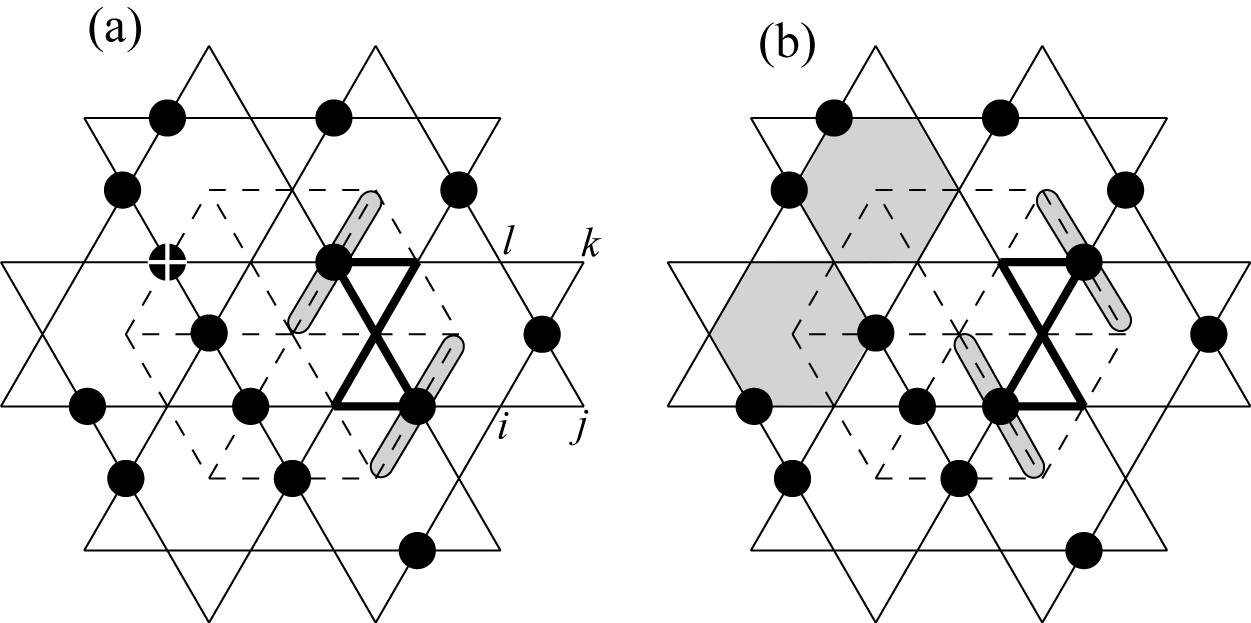
\includegraphics[width=6in]{kagome}
  \caption{ (a) Spins (black dots are $S^z = 1/2$) in a groundstate configuration satisfying $H_0$ on the kagome lattice.  The degenerate manifold of such configurations maps onto a triangular-lattice (dashed) classical three-dimer configuration, where each spin-up corresponds to a dimer on the dual lattice \cite{BFG}.  (b) At right, a plaquette-flip $H_{\rm ring}$ operation preserves the cluster-charging constraint, and can be seen to correspond to a rhombus-flip of dimers on the dual lattice.  A defect is created by flipping one spin (marked ``+'' in (a)).  This defect can be thought of as associating with two hexagonal plaquettes (grey in (b)), each with two spin-up per hexagon, corresponding to deconfined fractionalized spinons.} \label{kag_fig}
\end{figure}

The recipe to construct QSL phases in XXZ spin (or boson) models is to map the dimer constraint to a plaquette spin configuration on the dual lattice; the dimer may represent an $S^z$ spin configuration on a bond which is frustrated (or unsatisfied).  Then, the role of the quantum dimer tunnelling moves is done by a spin-exchange processes (which may {\it not} be a simple two-body term).  Such models have been called
{\it cluster-charging} models \cite{Isakov2}, because spin configurations summed over a local cluster (e.g.~a lattice plaquette) are penalized when differing from some chosen value.  For example:
\begin{eqnarray}
%H &=& -t \sum_{\langle ij \rangle} [b^{\dagger}_i b_j + b_i b^{\dagger}_j] + V \sum_{\hexagon} (n_{\hexagon})^2 \\
%H_0 &=& -t \sum_{( ij )} [b^{\dagger}_i b_j + b_i b^{\dagger}_j] + V \sum_{\hexagon} (n_{\hexagon})^2 
H_0 &=& V \sum_{\hexagon} (S^z_{\hexagon})^2 
\end{eqnarray}
with $S^z_{\hexagon} = \sum_{i \in \hexagon}S^z_i$,
is a cluster-charging potential term which favors three spin up and three spins down per hexagonal plaquette.  This Hamiltonian alone will promote a highly degenerate manifold of groundstate configurations, where each lattice hexagon satisfies the plaquette constraint but is otherwise disordered.  
Like all Hamiltonian operators which are entirely diagonal in the QMC basis, $H_0$ does not affect the simulation with a sign problem, no matter how the interaction is frustrated.

In order to promote a QSL phase from this classical degenerate manifold, one desires to add quantum fluctuations to this Hamiltonian such that the cluster-charging constraint is not violated.  In this case, a {\it ring-exchange} term, 
\begin{eqnarray}
%H_{\rm ring} = -K \sum_{\bowtie} ( b_i^{\dagger} b_j^{\phantom\dagger} b_k^{\dagger} b_l^{\phantom\dagger} + {\rm h.c.} )
H_{\rm ring} = -K \sum_{\bowtie} ( S_i^{+} S_j^{-} S_k^{+} S_l^{-} + {\rm h.c.} )
\end{eqnarray} 
promotes quantum fluctuations while preserving the cluster-charging constraint $H_0$.  Thus, one expects the kagome lattice model with $H = H_0 + H_{\rm ring}$ to retain a disordered groundstate with quantum fluctuations - a good candidate for a quantum spin liquid phase.  In addition, with $K>0$, such terms do not have the sign problem for QMC \cite{JKqmc}.

Balents, Fisher and Girvin \cite{BFG} were the first to show that variations of this kagome-lattice model support the simplest type of Z2 spin liquid -- in particular, at an exactly soluble Roksar-Kivelson point.  Subsequently, using QMC simuations, Isakov and co-workers showed that a variant of the cluster-charging Hamiltonian with different short-range exchanges: 
\begin{eqnarray}
H_{1,3} &=& -t_{1,3} \sum_{( ij )_{1,3}} [S^{+}_i S^-_j + S^-_i S^{+}_j]  
%H_0 &=& -t \sum_{( ij )} [b^{\dagger}_i b_j + b_i b^{\dagger}_j] + V \sum_{\hexagon} (n_{\hexagon})^2 
%H_0 &=& V \sum_{\hexagon} (n_{\hexagon})^2 
\end{eqnarray}
support a $Z_2$ spin liquid phase.  Again, for $t_{1,3}>0$ no sign problem exists.  This exchange term can either connect the first, second and third neighbors $( ij )_3$ on the kagome lattice \cite{Isakov1,Isakov2}; or it can be nearest-neighbor only $( ij )_1$ \cite{TopoEE}.  
%Because of the ability to simulate this class of Hamiltonian without the sign problem, several combinations of the above terms have recently been studied with large scale QMC, and demonstrated to have a Z2 spin liquid phase.  
In addition to  $H = H_0 + H_3$, $H = H_0 + H_1$, the $Z_2$ spin liquid has been demonstrated on $H = H_1 + H_{\rm ring}$, where the cluster-charging term is not explicitly required and the Hamiltonian consists of two competing kinetic-energy terms \cite{Long}, sometimes called the J-K model \cite{JKqmc}.

%The cluster-charging potential term is given by the interaction $V$, which favors 3 bosons per site.  Quantum fluctuations are proportional to $t$: they can be nearest-neighbor\cite{TopoEE} or have equal first, second and third nearest-neighbors\cite{Isakov1,Isakov2}.  This model maps to the three-dimer model on the dual lattice...

%These examples are part of a broader class, originally identified to harbour the simplest Z(2) spin liquid phase at an exactly soluble RK-point, was introduced by Balents, Fisher and Girvin.\cite{BFG}  

In the next section, we explore one procedure by which QMC simulations can positively identify such spin liquid phases.  In section \ref{XYstar}, we examine the FM (or ``superfluid'' in the boson language) to QSL phase transition, which is common to these models, as an different example of a deconfined or fractionalized quantum critical point.

\subsection{Identifying the $Z_2$ spin liquid: Topological Entanglement} \label{topoEEsec}

The smoking gun signature for a gapped spin liquid phase could be argued to be the identification of an emergent gauge theory,
and the associated topological order.  One manifestation is the existence of a ground state degeneracy, which is topological in nature, in the simplest ($Z_2$) case being four-fold on a torus.  Previous QMC studies of QSL states have demonstrated the difficulty in clearly identifying this degeneracy, due to the tendency for tunnelling between the equal-energy states on finite-size lattices with physical Hamiltonians \cite{Isakov1}.  Similarly, recent DMRG work purporting to identify candidate gapped spin liquid states have been unable to identify the associated topological degeneracy \cite{Yan,J1J2}.

Luckily, the community has another tool suited for the positive identification of this topological order, through measurements of the Renyi entanglement entropy, introduced in section \ref{ss:renyi}.  The $S_{\alpha}$ are well-studied quantities in quantum information science; they quantify correlations for a system in a basis-independent way, which makes them suitable in particular for characterizing phases that do not have an explicit broken symmetry (in particular QSL phases).  In fact, some authors have championed the entanglement entropy as a paradigmatic analog to symmetry breaking for non-Landau phases; here, the concept of {\it Long Range Entanglement} (LRE) replaces the concept of {\it Long Range Order} (LRO) \cite{Wenbook}.  For example, in a gapped phase with LRO (such as the VBS phases mentioned above),
the entanglement entropy is expected to obey the ``area law''
\begin{equation} 
S_{\alpha} = a\ell + \cdots
\end{equation}
where $a$ is a non-universal constant, $\ell$ is the length of the boundary between regions $A$ and $B$, and terms denoted by $\cdots$ scale away at least as fast as $\mathcal{O} (1/\ell)$.  This can heuristically be considered as ``short-range'' entanglement.  In contrast, in a gapped spin liquid phase (with no broken symmetries)
scaling of entanglement entropy is predicted to be
\begin{equation}
S_{\alpha} = a \ell - \gamma + \cdots \label{areaL}.
\end{equation}
 Here, the subleading term to the area law is a universal correction called the {\it topological entanglement entropy} \cite{Alioscia1,Alioscia2,LW,KP}.  In a gapped quantum spin liquid phase, it is related to the emergent gauge symmetry (independent \cite{Flammia} of Renyi index $\alpha$), e.g.~in the $Z_2$ spin liquid state $\gamma =  \ln(2)$ at $T=0$ \cite{LW}.   The addition of a universal subleading constant to the area law motivates the notion of LRE for a quantum spin liquid phase.


Using the estimators described in Section~\ref{ss:renyi}, it is possible to isolate the topological entanglement entropy from the leading-order area-law, as well as subleading corrections due to effects such as corners, by taking measurements using several different geometries $A$ and performing additions or subtractions which isolate only $\gamma$.  For example, the {\it Levin-Wen} \cite{LW} regions isolate $2\gamma$ from Eq.~(\ref{areaL}), requiring measurement of four unique region $A$ geometries.  For a BFG Hamiltonian discussed in the last section, it is possible to extract the topological entanglement entropy in a QMC simulation.  As noted by Castelnovo and Chamon \cite{castelnovo} through direct calculation on the toric code (which realizes a $Z_2$ fractionalized spin liquid groundstate), the value of $2\gamma$ is approached through two temperature crossovers on a finite-size system, related to the energy of the quasiparticle excitations in the groundstate -- one $Z_2$ charge corresponding to the spinon; one $Z_2$ flux corresponding to the vison.  Each excitation contributes a value of $\ln(2)$ to the topological entanglement entropy.  As illustrated in Figure \ref{QSLfig}, the realization of one of these plateaus at finite-temperature gives positive identification that the groundstate of the model is a $Z_2$ QSL phase.

\begin{figure}
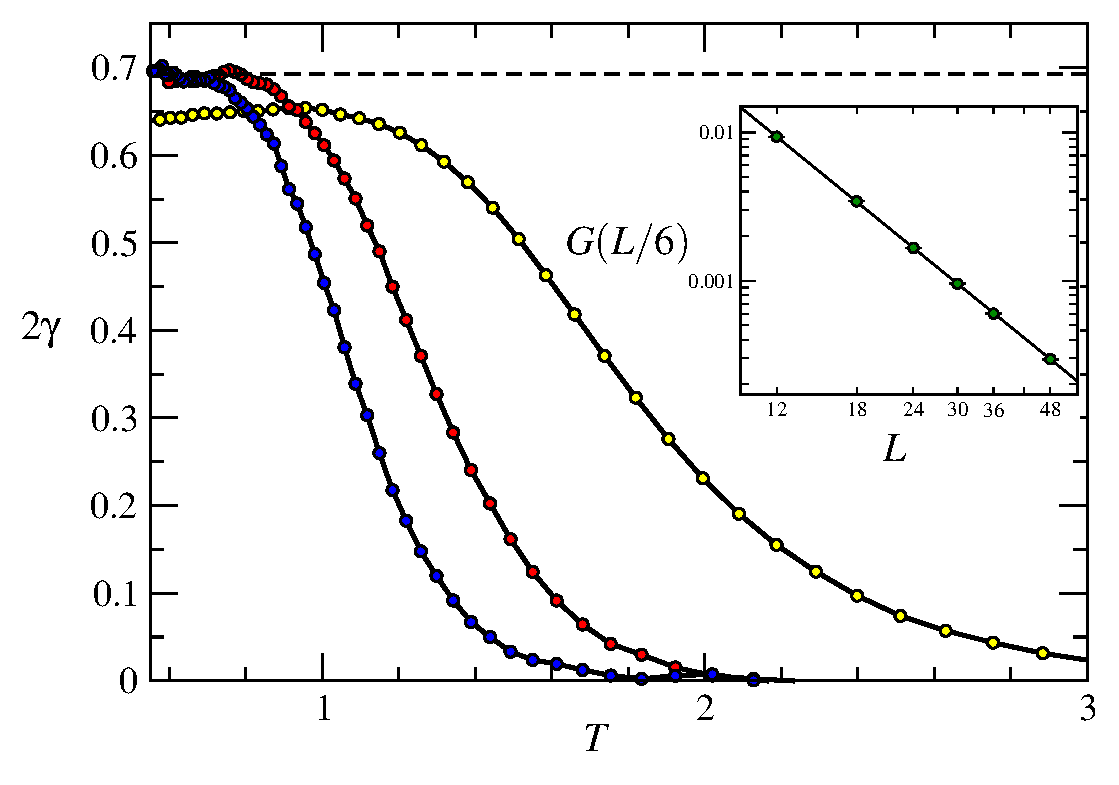
\includegraphics[width=5.5in]{QSL}
\caption{In the main figure, the temperature dependence of the topological entanglement entropy in the $Z_2$ QSL phase of the Hamiltonian $H_0 + H_1$ (reproduced from \cite{TopoEE}), for three different sizes of kagome lattice.  The quantization of the plateau at $\ln(2)$ (dashed line) identifies the emergent gauge symmetry; at $T=0$ one expect another temperature crossover to $2 \gamma = 2 \ln(2)$.  In the inset, finite-size scaling of
$G(L/6)$ at the XY* quantum critical point, which scales as  $1/L^{2.493}$ (straight-line fit) giving $\eta = 1.493$ (reproduced from \cite{XYstarQMC})
\label{QSLfig}}
\end{figure}

Interestingly, the existence of the $Z_2$ fractional phase in the kagome BFG Hamiltonian also raises the possibility that, with a suitable ``binding'' potential \cite{FermionBind}, an extension of the model with an emergent fermionic excitation might be created \cite{Wenbook}.  
Future QMC simulations on designer Hamiltonians will be required to address the interesting question of whether fermions can be observed emerging as collective excitations of a purely bosonic microscopic model without the sign problem.

\subsection{Deconfinement at the XY* transition} \label{XYstar}

The fractional spinons of the $Z_2$ spin liquid phase (illustrated in Fig.~\ref{kag_fig}) can be thought of as a ``square-root'' operator of the physical spins.  Employing the mapping from $S^z$ spins to hard-core bosons, we can relate the physical spin $S^+$ or (equivalently) boson operator $b^{\dagger}$ as being composed of two operators  $\phi^\dagger \phi$, where $\phi^\dagger$ and $\phi$ denote the raising and lowering operators for the fractionalized spinon particles.  
Surprisingly, it is predicted that the quantum phase transition between the XY-ferromagnet and the $Z_2$ spin liquid discussed in the last section can actually be mediated not by the physical bosons (which would undergo a quantum phase transition in the 3D XY universality class), but by the fractional spinon fields \cite{XYstar1,XYstar2,earlyXYstar}.  This leads to the same exponents $z$ and $\nu$ as in the ordinary $XY$ critical point.  However, the exponent $\eta$ controlling the equal time correlation function $\langle b^\dagger(0) b(x) \rangle$ is modified as mentioned in Section~\ref{ss:j1j2N}, such that one expects a large $\eta \approx 1$.

Previous estimates for $\eta$ were obtained from field-theoretic treatments.  From $1/N$ expansion, Ref.~\cite{XYstar2} obtains
\begin{equation}
\eta = 1 + \frac{32}{3 \pi^2 N}
\end{equation}
which gives $\eta = 2.08$ for $N=1$.
A more accurate value was obtained from a combination of field theoretic and Monte Carlo simulations of the correlation of a composite operator in the 3D XY model\cite{compositefieldtheory,compositeMC}, leading to $\eta\approx  1.47(3)$.

The measurement of $\eta$ in the kagome BFG model is challenging, requiring measurement the equal time Green's function in real space: $G(x)\equiv G(\tau=0,r) = \langle b^\dagger(0) b(r) \rangle$ \cite{WormA,gfsse}, done by keeping track of the defects created in the loop algorithm \cite{Syljuasen02} as it traverses the QMC's $d+1$ space-time simulation cell.  At the critical point, $G(r)$ should decay as $1/r^{1+\eta}$, and finite size effects can be minimized e.g.~by measuring $G(L/6)$, which decays as $1/L^{1+\eta}$, as a function of $L$.  Fig.~\ref{QSLfig} show an algebraic decay with $\eta=1.493(10)$, a value that is consistent with $\eta$ for a composite operator in the 3D XY model.  The excellent agreement between QMC simulation results and the composite boson field theory is a remarkable confirmation of fractionalized universality in this model; synergetic work between QMC and quantum field theory is uniquely capable of positive identification of exotic quantum phase transitions in this model.

As discussed in Ref.~\cite{XYstarQMC}, there are consequences of this novel fractionalization in other universal quantities.  Remarkably, even though the fractional excitations become gapless at the quantum critical point, there are still observable remnants of the topological nature of the $Z_2$ spin liquid.  This can be seen by looking at the winding number distribution at the XY* point, and comparing it to the winding number distribution at a regular 3D XY transition.  Namely, since the fractional spinons are bosonic, they can be modelled by a ``simulation within a simulation'', achieved by projecting physical bosons at an XY transition to wind strictly in pairs around the periodic simulation cell.  Since this distribution is universal, it is expected to be the same (up to a non-universal velocity) as the winding number distribution of the physical (composite) bosons in the XY* transition.  Observation of this fact \cite{XYstarQMC} is a striking confirmation that topological properties can still be present even when fractional excitations are gapless.  These universal winding number distributions are possible to compute in principle in field theory; hence they are another example that synergetic work between and quantum field theory and simulation is often led by the latter.


%\begin{enumerate}
%\item We have 4 or 5 Hamiltonians (with Z2 \cite{Isakov1} and U(1) spin liquids)
%\item Balents Fisher Girvin gave us a ``recipe'' for creating Hamiltonians with Z2 spin liquids using constrained interactions
%\item The connection to field theory is the emergent gauge structure I guess
%\item Entanglement entropy identifies the emergent gauge structure of the underlying theory
%\item XY*
%\end{enumerate}

\section{Discussion}
\label{sec:discussion}

We have here given some examples of what can be accomplished with judiciously constructed designer Hamiltonians. Here we discuss
some further generic aspects of this approach, followed by an outlook on future directions.

\subsection{Designer hamiltonians, stoquasticity, and the sign problem}

The concept of designer Hamiltonian we have introduced here is different from the ``stoquastic'' Hamiltonians \cite{Terhal08}; 
those for which all off-diagonal matrix elements are non-positive (i.e., sign-problem free) in the standard basis, normally the standard $z$-component 
basis for spin systems [although a broader definition with respect to an arbitrary basis has also been presented \cite{Terhal09}, which would seem to 
indicate that any Hamiltonian could in principle be cast into this class]. Our criterion is more one of scientific utility than a strict mathematical 
definition---models that are free from sign problems either automatically (i.e., they are stoquastic in a practically useful basis), or through some 
other way of circumventing it [i.e., the Meron algorithm \cite{Chandrasekharan99} or determinant-based QMC of particle-hole symmetric Hubbard 
models \cite{White89,Assaad05,Assaad07}]. Importantly, to be considered a designer Hamiltonian, such a model should also represent a prototypical case of 
some interesting quantum-man body phenomenon which is difficult to access in an unbiased manner in other ways, i.e., the model is designed to shed
light on this problem (and must be ``de-signed'' to be practically useful for studies on large scale).

An important fundamental problem is whether it is always possible to construct such designer hamiltonians, or whether certain types of 
states is beyond reach in practice because their physical properties are fundamentally tied to the difficulties in curcumventing the sign problem. 
The $Z_2$ spin liquid [which itself is a broad class if states \cite{Wen03}] in SU($2$) variant models is potentially an example of such a state. 
It is certainly possible that such a state cannot be realized with stoquastic hamiltonians in a simple basis, but one can still not exclude that 
designer hamiltonians can be constructed for which some useful basis can be found, or for which the sign problem can be solved in some other way.
Indeed, the recent discovery of a spin liquid in the Hubbard model on the honeycomb lattice \cite{Meng10} seems to provide an example, although it 
remains to be seen whether this state really is a $Z_2$ topological state.

Regarding the sign problem itself more broadly, Ref.~\cite{Troyer05} presents a proof that the sign problem cannot be solved in general. 
The problem is here defined in terms of constructing a QMC algorithm for which the computational effort scales as a power-law in the system
size. They show a particular problem for which the removal of the sign still leaves a problem for which the Monte Carlo sampling is believed 
to scale exponentially in the system size. However, the problem chosen is that of a spin glass, and the conclusion reached is equivalent to
the statement that the quantum spin glass is not easier to solve than the corresponding classical spin glass. This is hardly a surprising result, 
and the proof does not say anything about QMC solutions of systems that are not directly associated with the well known difficulties of simulating 
classical glassy systems with complicated energy landscapes. Whether or not the sign problem can be circumvented (at least for representative 
designer hamiltonians) for translationally invariant systems such as fermionic Hubbard models without particle-hole symmetry and SU($2$) frustrated 
quantum spins models remains and open question.

\subsection{future prospects}

Within the classes of models we have discussed here, although the essential physics is now has been assertained, there still remains
important work to be done to improve on the quantitative aspects, e.g., the critical exponents. In the case of the studies aiming to connect
SU($N$) QMC simulations with large-$N$ expansions, summarized in Sec.~\ref{sec:sunmodels}, it would be very useful to go to still larger lattices, 
to investigate the convergence of the computed exponents. This is importan, in particular, in light of the fact there there are significant scaling 
corrections in quantities such as the spin stiffness for $N=2$. Such corrections could potentially affect also the fitting procedures underlying 
the exponents graphed in Fig.~X for small N. When higher-order $1/N$ analytical results eventually become available, it will be important to know 
the values of the exponents without possible remaining effects of scaling corrections. What is needed here is high-accuracy (small error bars) 
results for the correlation functions on large lattices.

- Fermions: it should be possible to study 1 or 2 fermions (manageble sign problem) in 
VBS/critical/spin-liquid systems. One should be able to see some aspects of the "strange metal''.
Mention meron algorithm---perhaps some more interesting designer hamiltonian can be constructed.

- Non-equilibrium QMC

- Using entanglement entropy to characterize non-Landau quantum critical points


\bibliography{rev_bib.bib}
\bibliographystyle{Science}

\end{document}

